\subsubsection{Sample size (Surrogate size) 1000 }
In this section we calculated flamespeed values for 1000 different points in the domain and the remaining values are linear combination of these 1000 points.  The results below are for sample size $1e5$, $5e5$ , $1e6$, $5e6$ and $1e7$. 

\begin{figure}[H]
\centering
\subfloat[MCMC raw chain of samples\label{subfig-1:dummy}]{%
     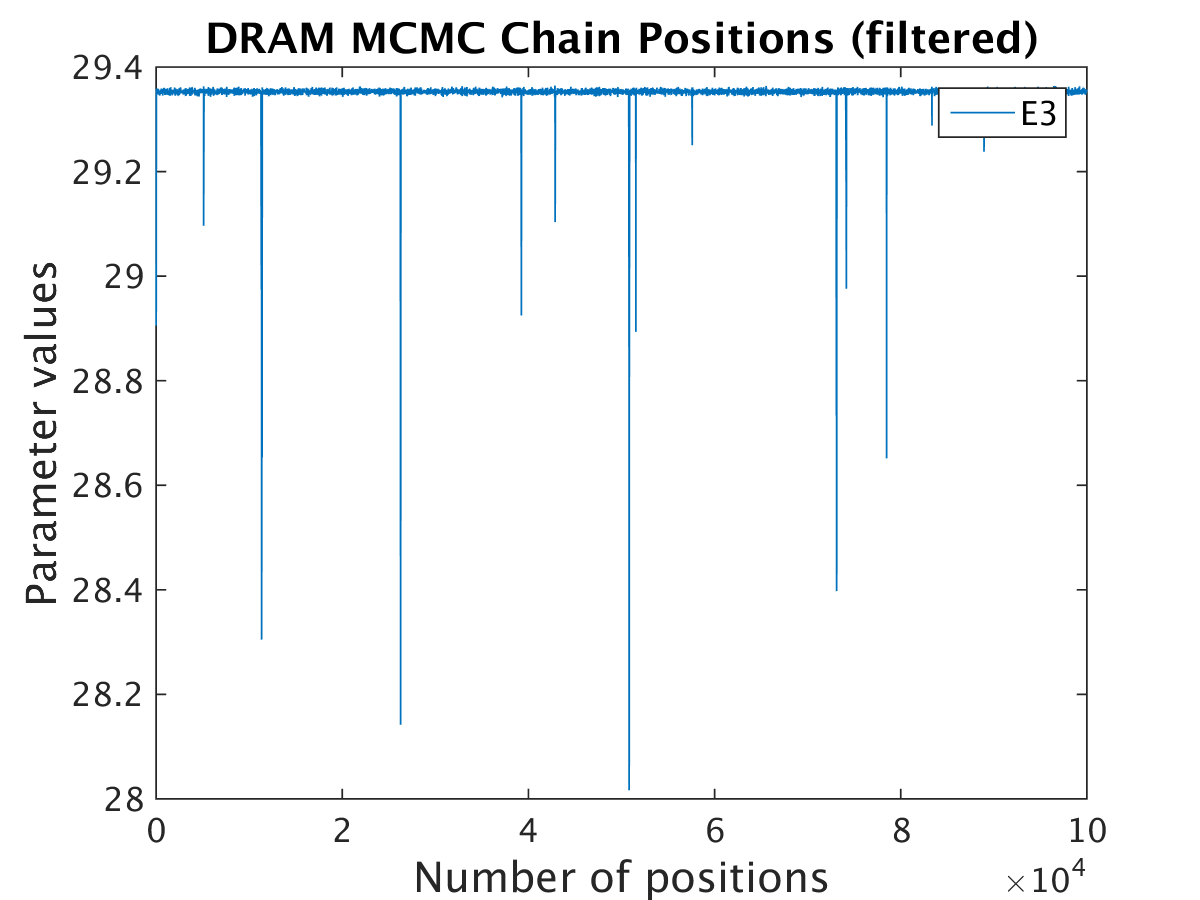
\includegraphics[scale=0.7]{one_parameter/1000_kde/outputData_1e5/simple_ip_chain_pos_filt} 
    }
    \quad
\subfloat[Histogram\label{subfig-1:dummy}]{%
     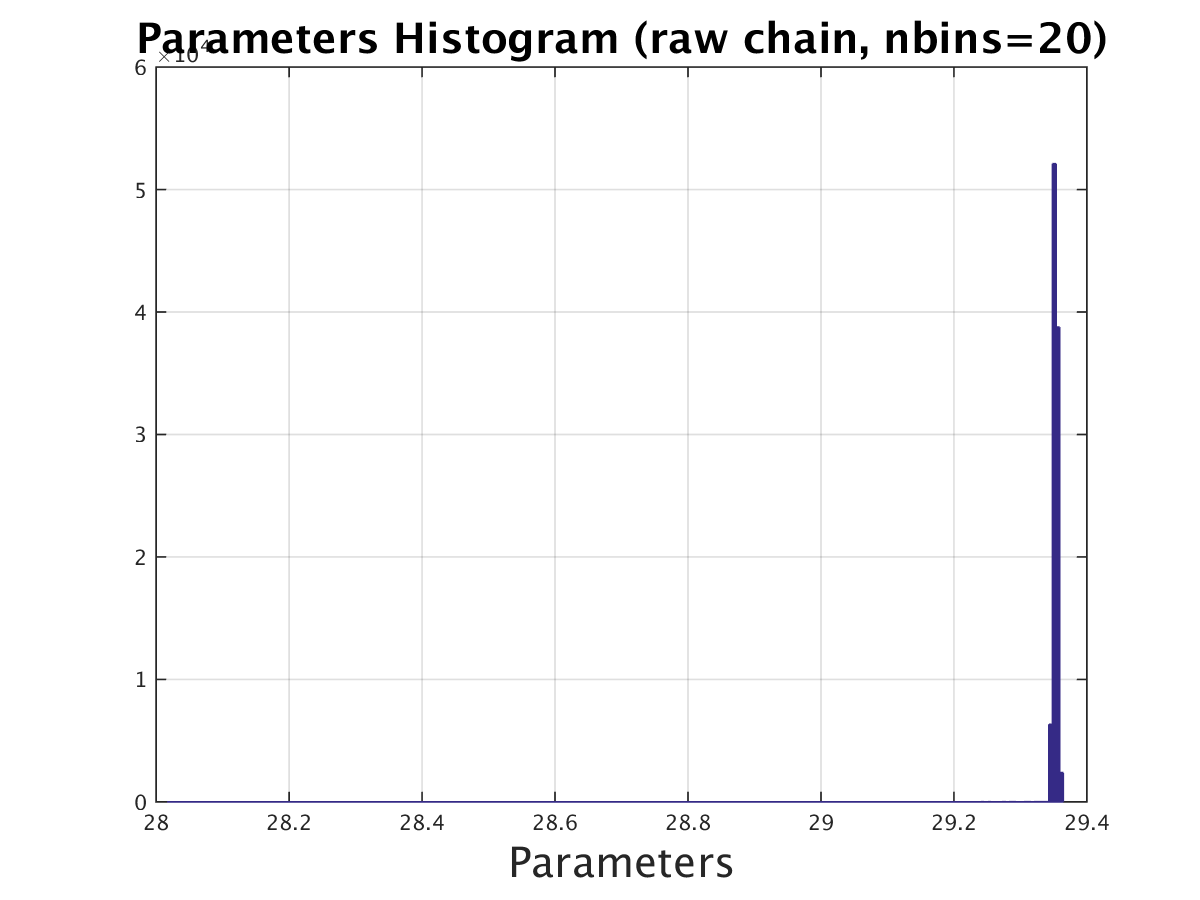
\includegraphics[scale=0.7]{one_parameter/1000_kde/outputData_1e5/simple_ip_hist_raw} 
    }
    \end{figure}
  \begin{figure}[H]
  \ContinuedFloat
  \centering
   \subfloat[Cummulative Density Funtion \label{subfig-1:dummy}]{
        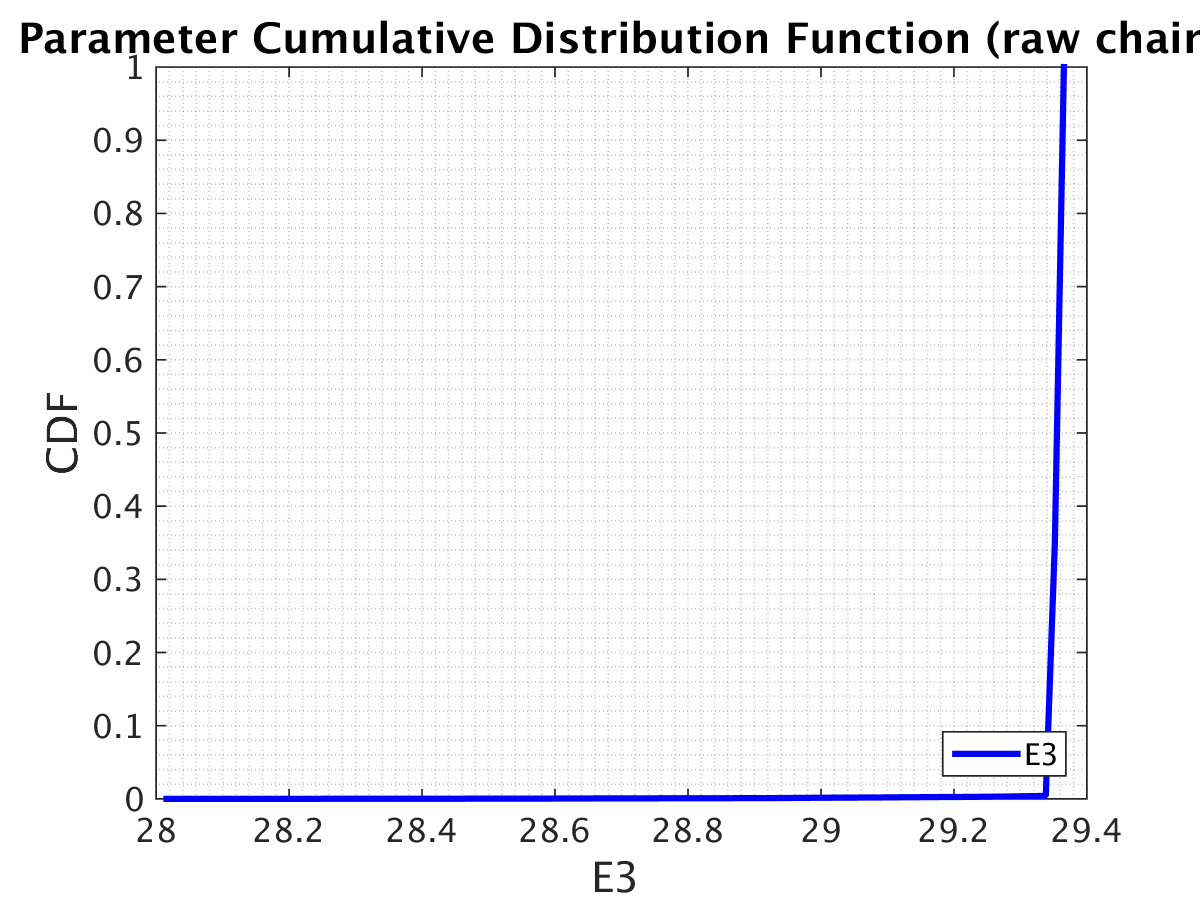
\includegraphics[scale=0.7]{one_parameter/1000_kde/outputData_1e5/simple_ip_cdf_raw} 
       }
     \quad
\subfloat[KDE \label{subfig-1:dummy}]{
        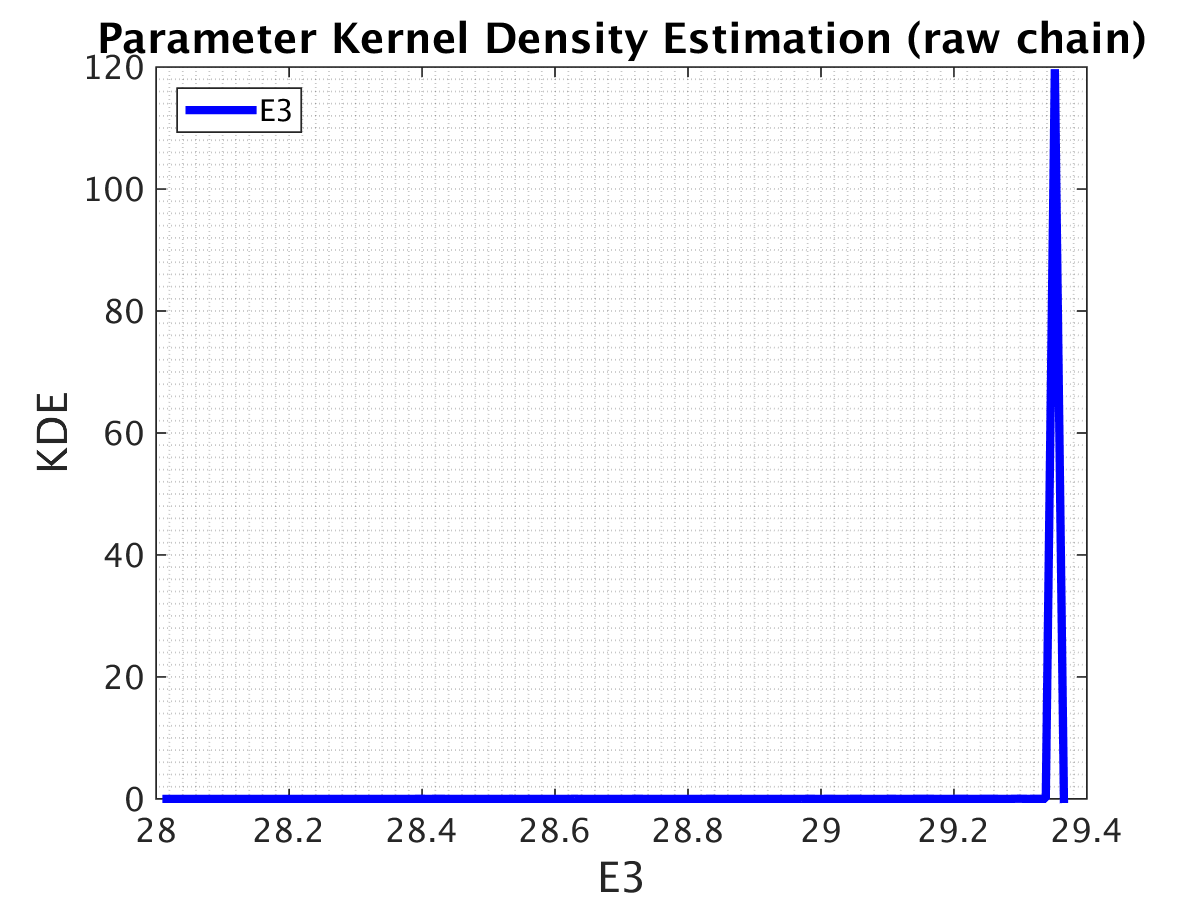
\includegraphics[scale=0.7]{one_parameter/1000_kde/outputData_1e5/simple_ip_kde_raw} 
            }  
\end{figure}
\begin{figure}[H]
 \ContinuedFloat
\centering
\subfloat[LogLikelihood \label{subfig-1:dummy}]{
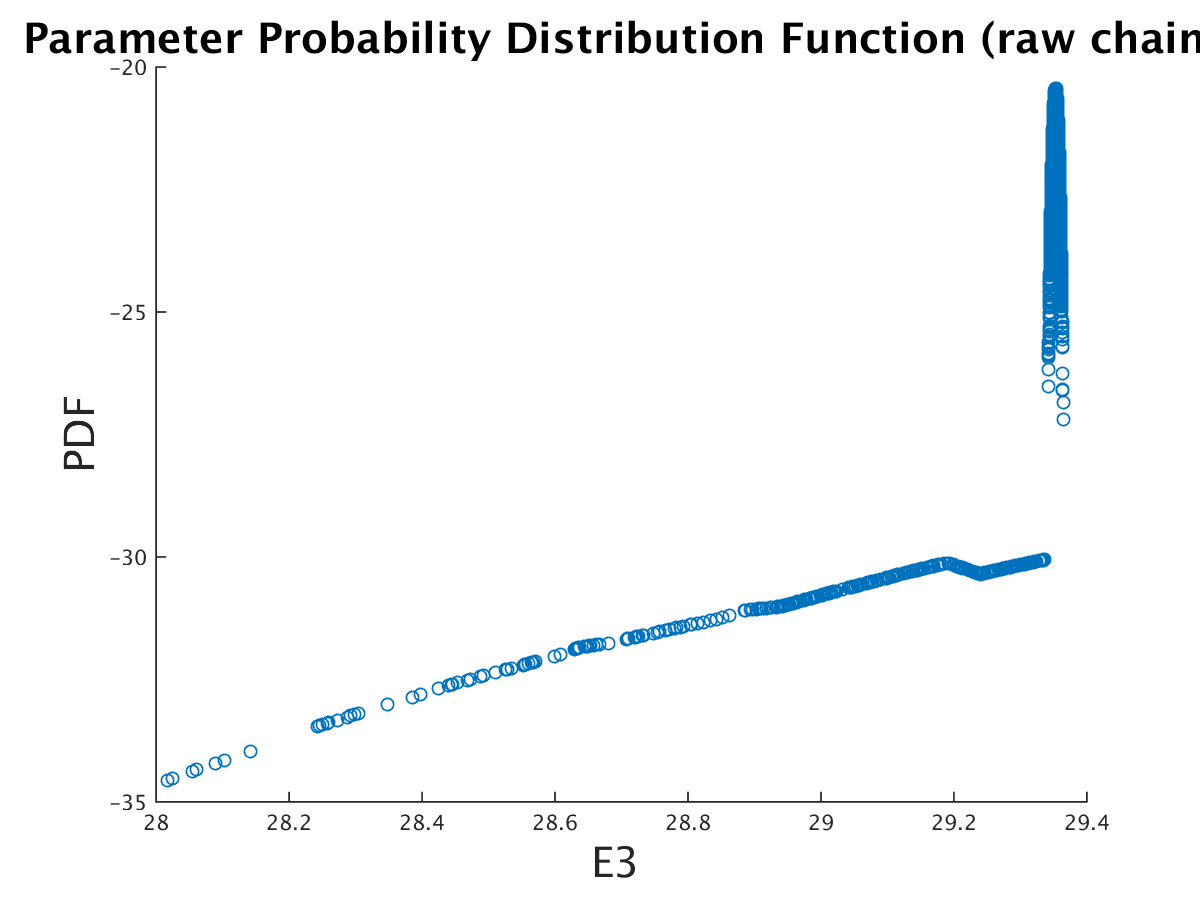
\includegraphics[scale=0.7]{one_parameter/1000_kde/outputData_1e5/ip_logLike_unified} 
  }
    \caption{Results for sample size 1e5}
\end{figure}

\begin{figure}[H]
\centering
\subfloat[MCMC raw chain of samples\label{subfig-1:dummy}]{%
     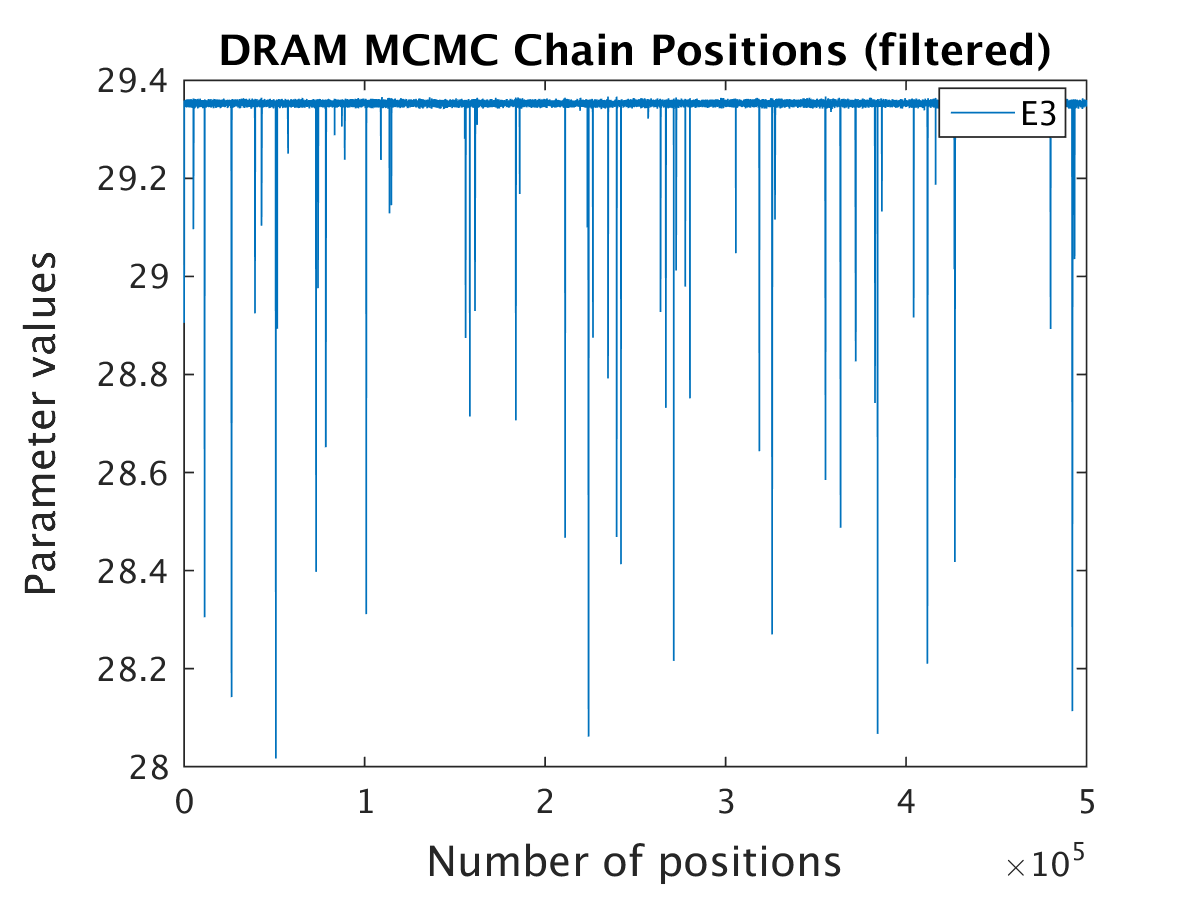
\includegraphics[scale=0.7]{one_parameter/1000_kde/outputData_5e5/simple_ip_chain_pos_filt} 
    }
    \quad
\subfloat[Histogram\label{subfig-1:dummy}]{%
     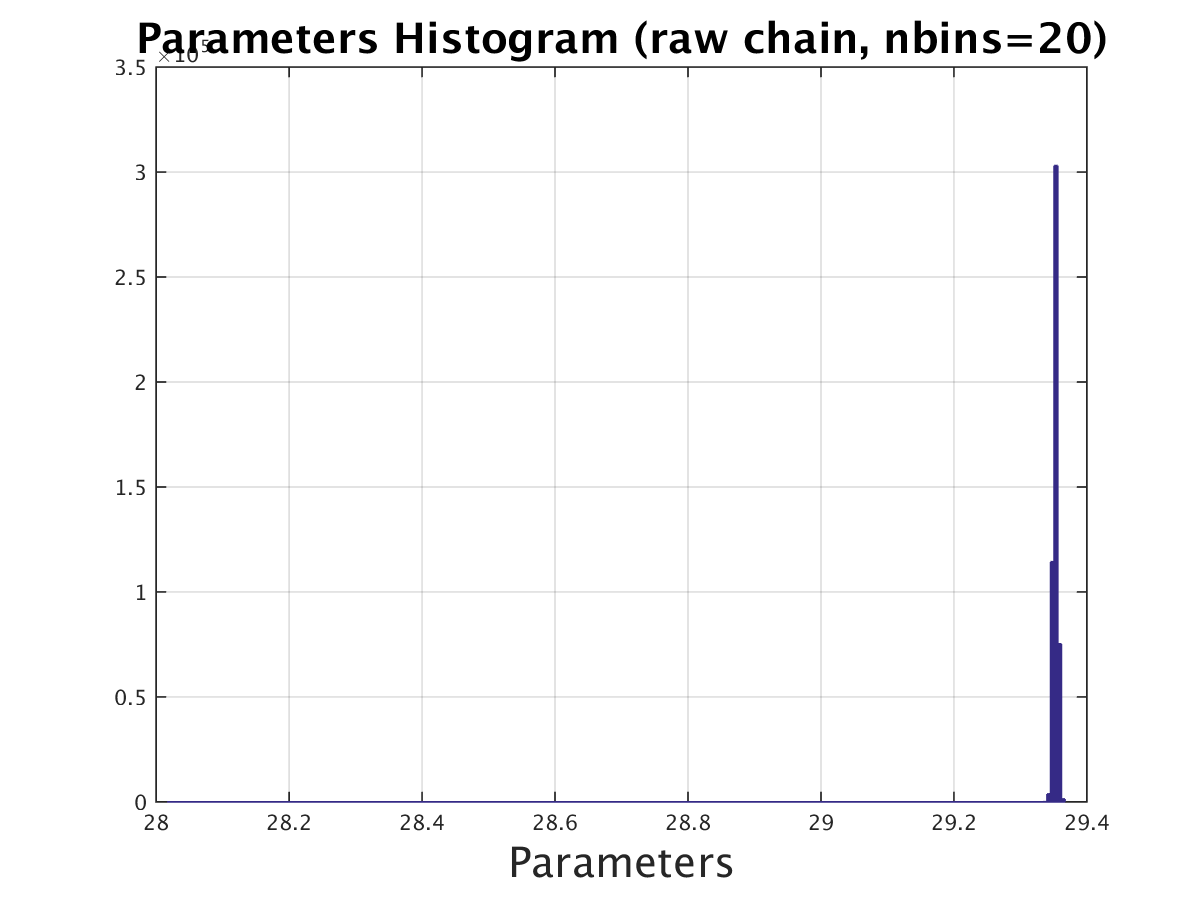
\includegraphics[scale=0.7]{one_parameter/1000_kde/outputData_5e5/simple_ip_hist_raw} 
    }
    \end{figure}
  \begin{figure}[H]
  \ContinuedFloat
  \centering
   \subfloat[Cummulative Density Funtion \label{subfig-1:dummy}]{
        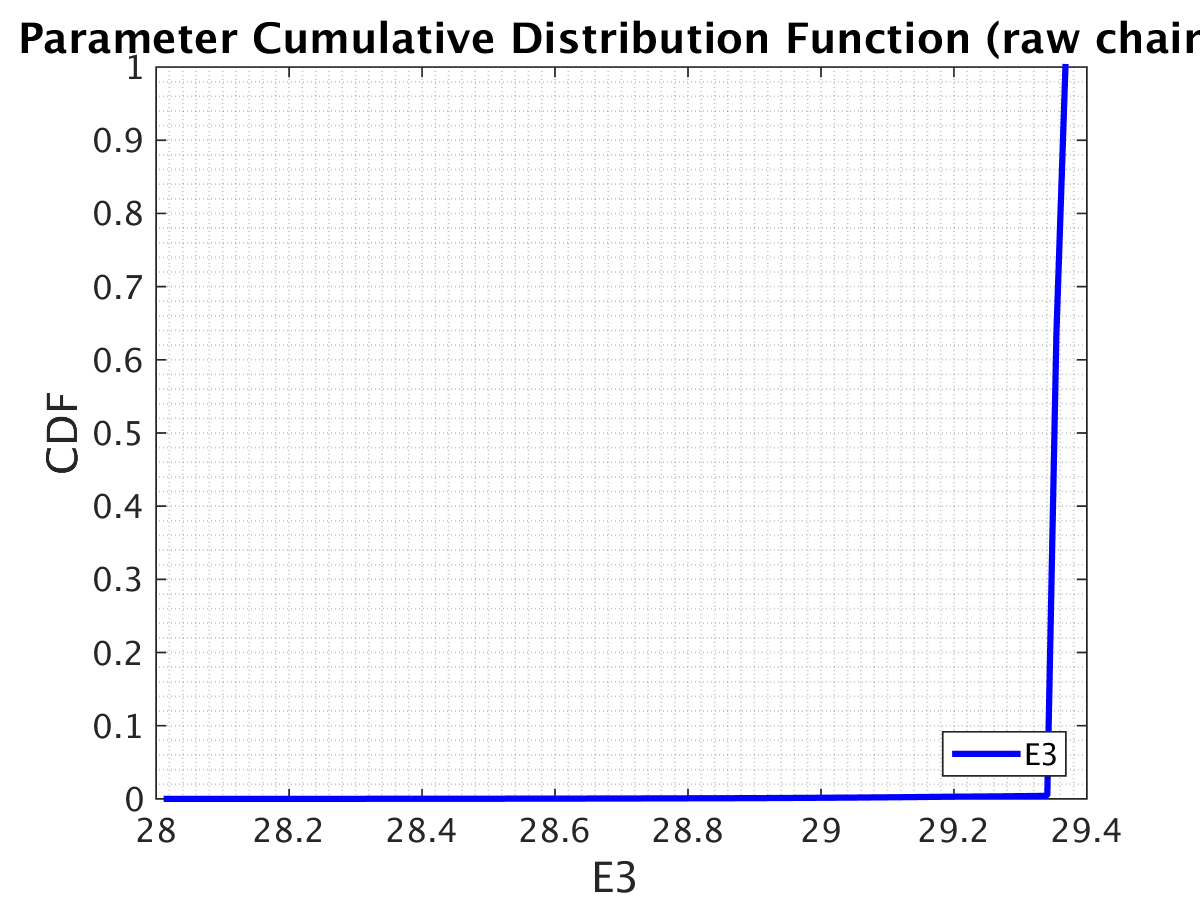
\includegraphics[scale=0.7]{one_parameter/1000_kde/outputData_5e5/simple_ip_cdf_raw} 
       }
     \quad
\subfloat[KDE \label{subfig-1:dummy}]{
        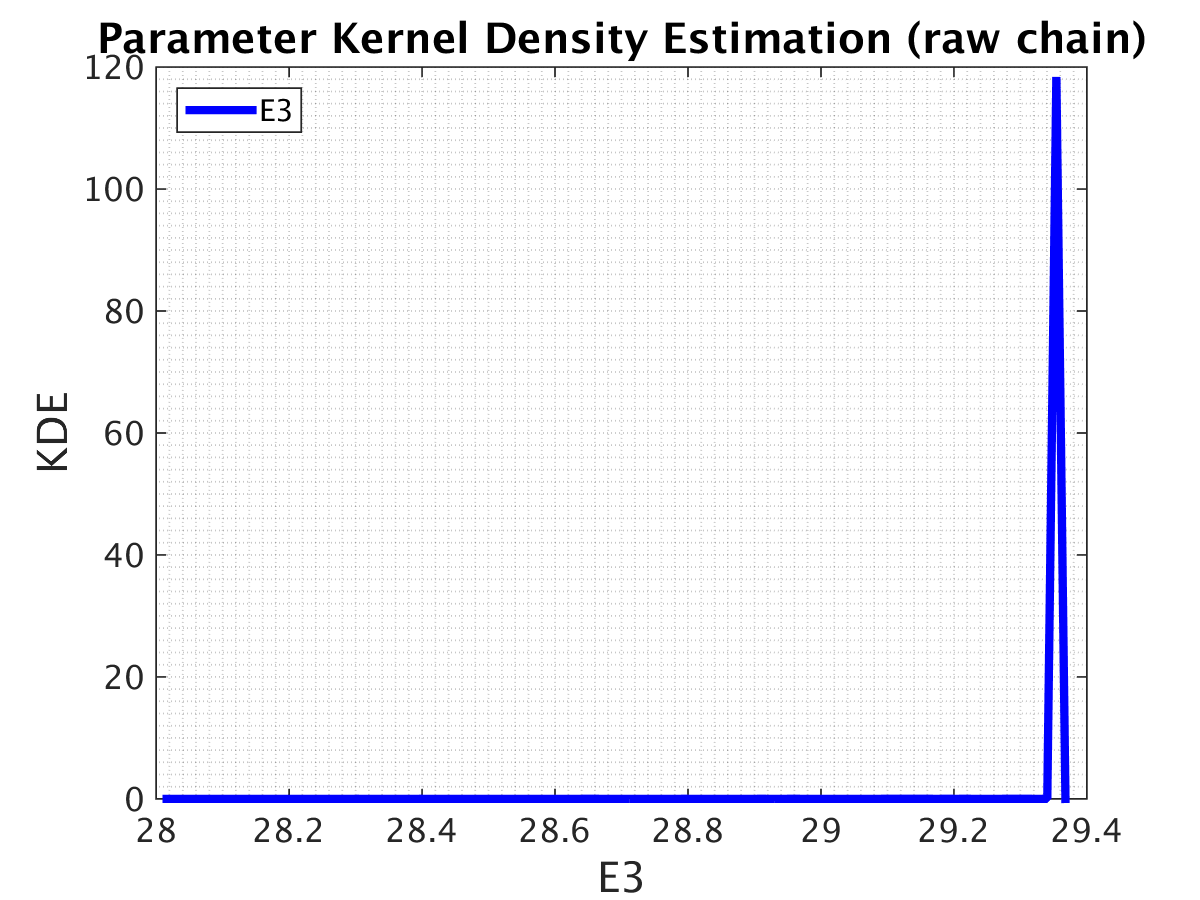
\includegraphics[scale=0.7]{one_parameter/1000_kde/outputData_5e5/simple_ip_kde_raw} 
            }  
\end{figure}
\begin{figure}[H]
 \ContinuedFloat
\centering
\subfloat[ LogLikelihood \label{subfig-1:dummy}]{
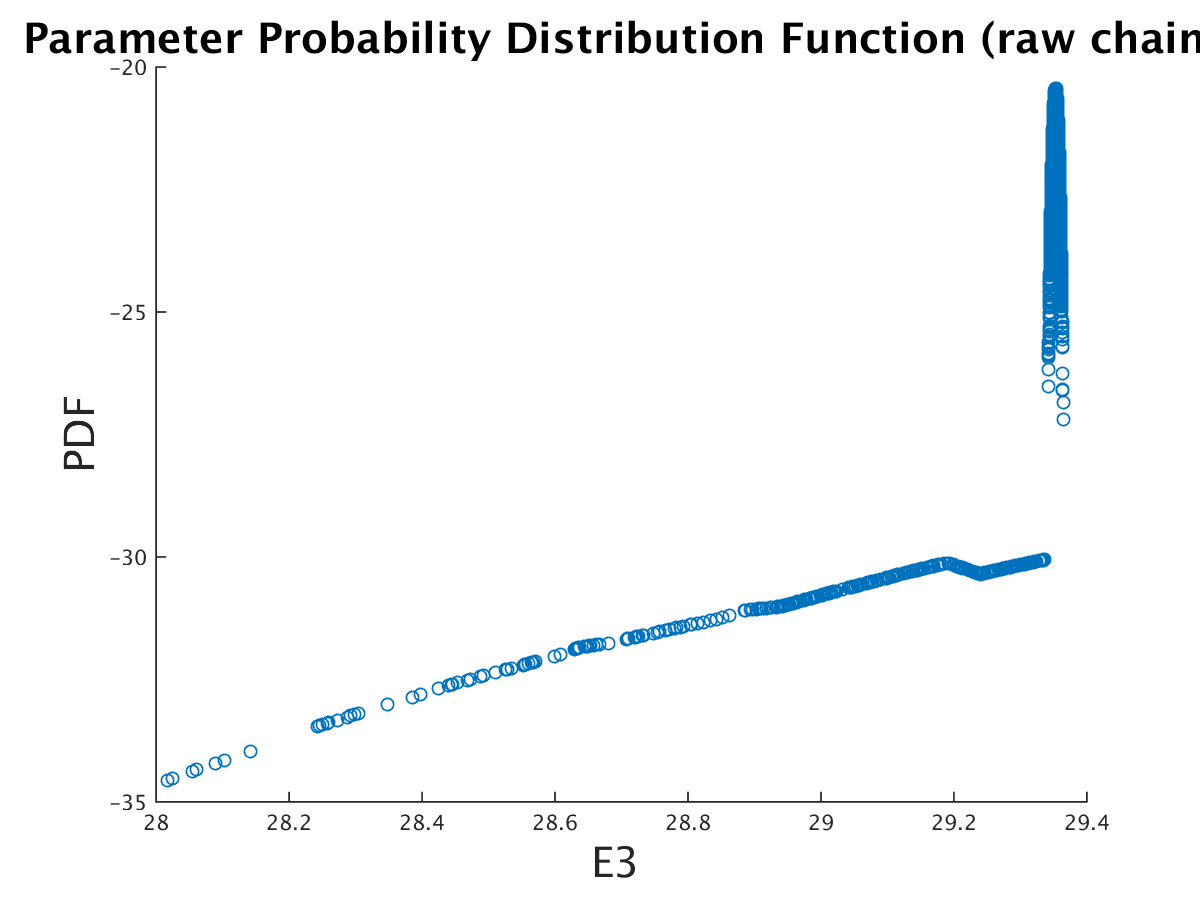
\includegraphics[scale=0.7]{one_parameter/1000_kde/outputData_1e5/ip_logLike_unified} 
  }
    \caption{Results for sample size 5e5}
\end{figure}


\begin{figure}[H]
\centering
\subfloat[MCMC raw chain of samples\label{subfig-1:dummy}]{%
     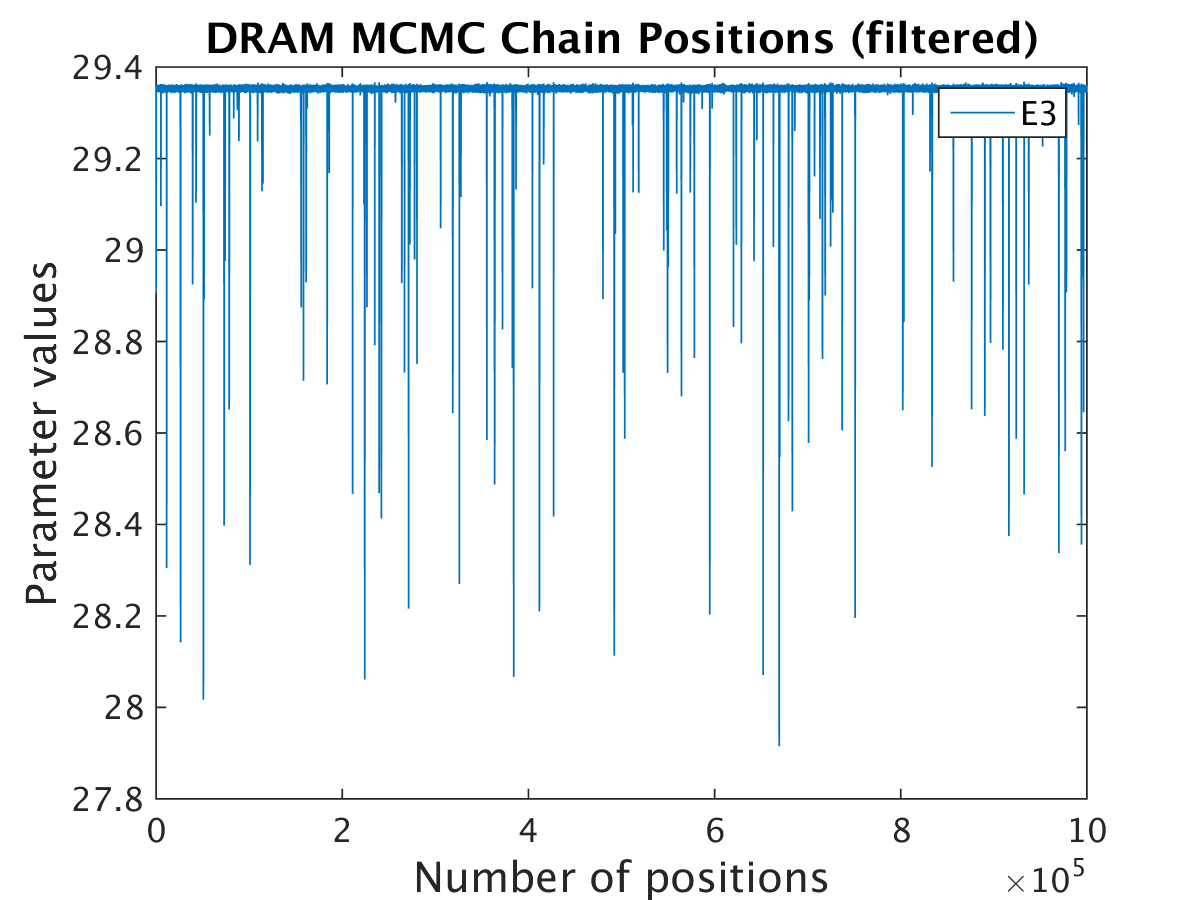
\includegraphics[scale=0.7]{one_parameter/1000_kde/outputData_1e6/simple_ip_chain_pos_filt} 
    }
    \quad
\subfloat[Histogram\label{subfig-1:dummy}]{%
     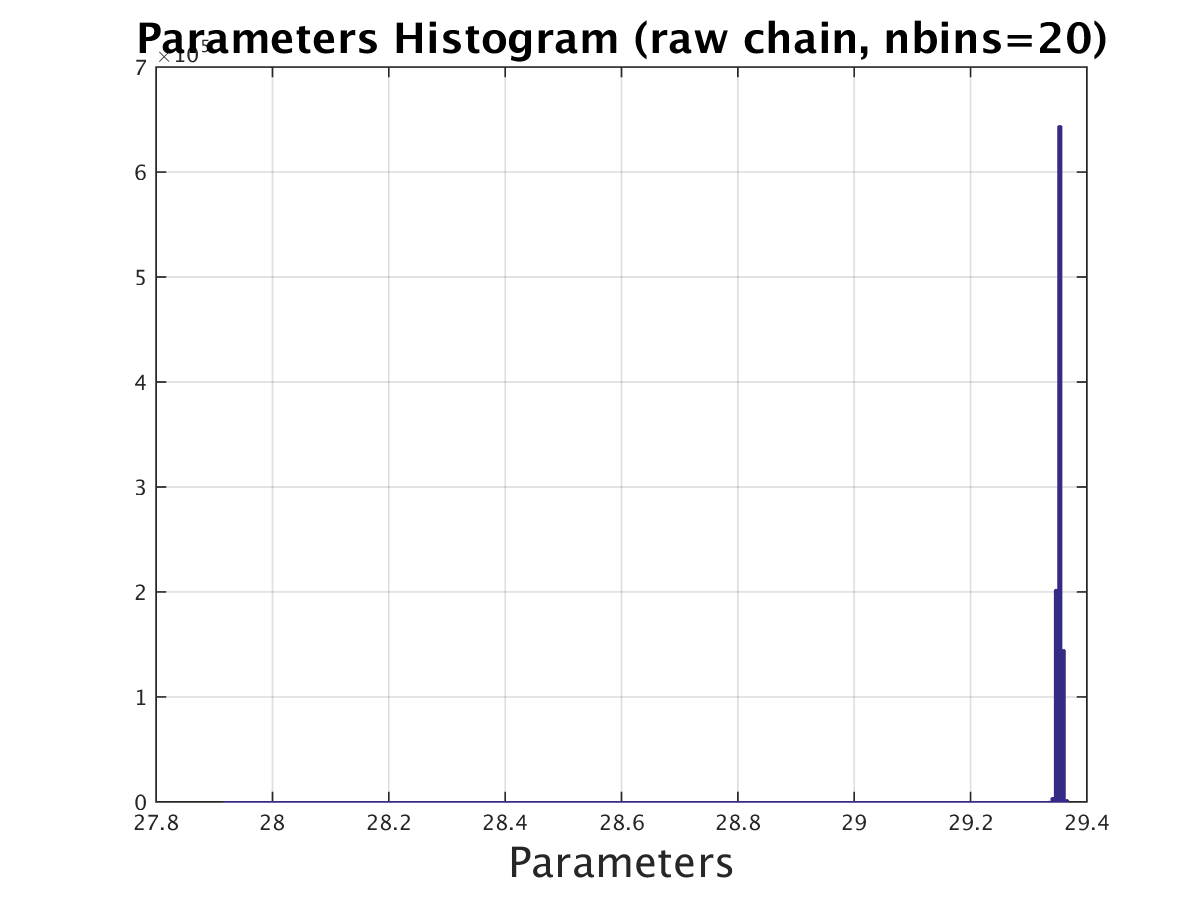
\includegraphics[scale=0.7]{one_parameter/1000_kde/outputData_1e6/simple_ip_hist_raw} 
    }
    \end{figure}
  \begin{figure}[H]
  \ContinuedFloat
  \centering
   \subfloat[Cummulative Density Funtion \label{subfig-1:dummy}]{
        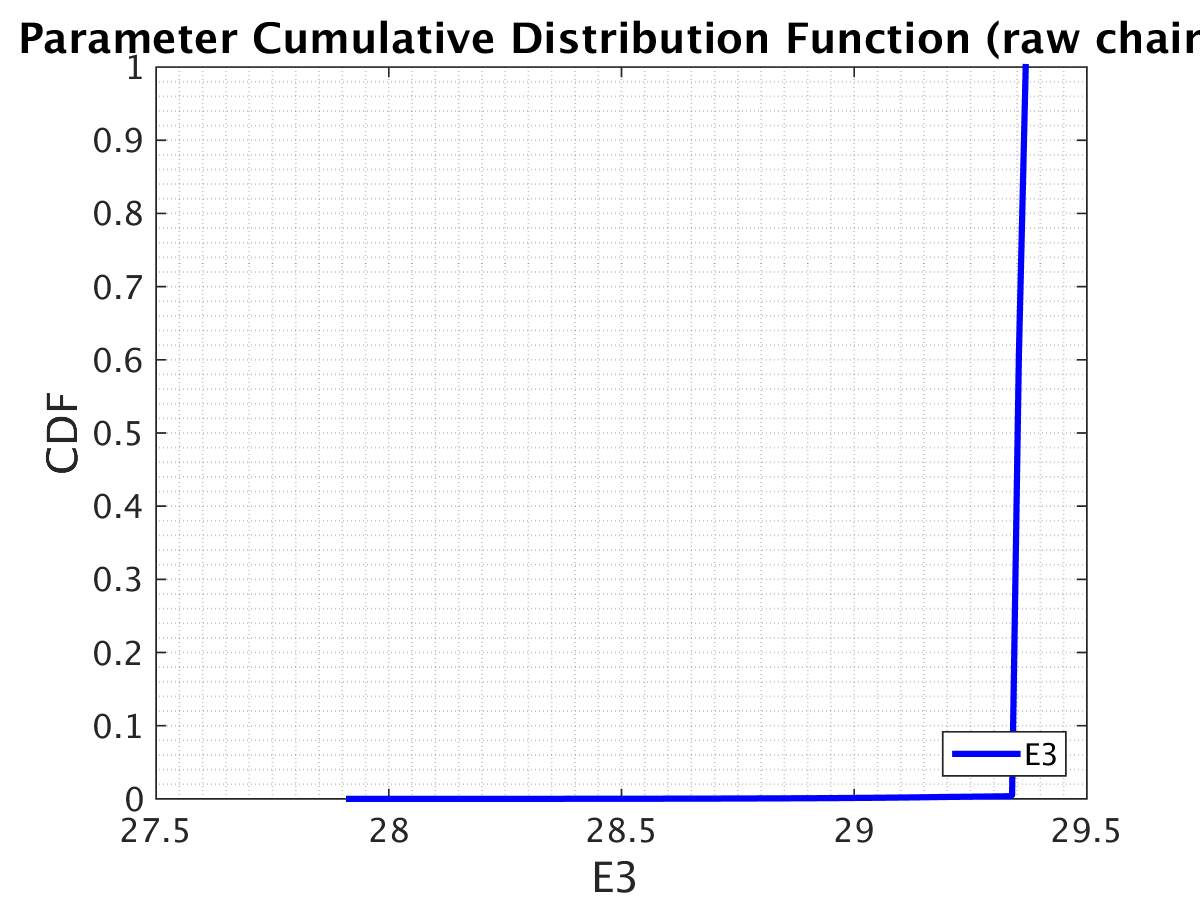
\includegraphics[scale=0.7]{one_parameter/1000_kde/outputData_1e6/simple_ip_cdf_raw} 
       }
     \quad
\subfloat[KDE \label{subfig-1:dummy}]{
        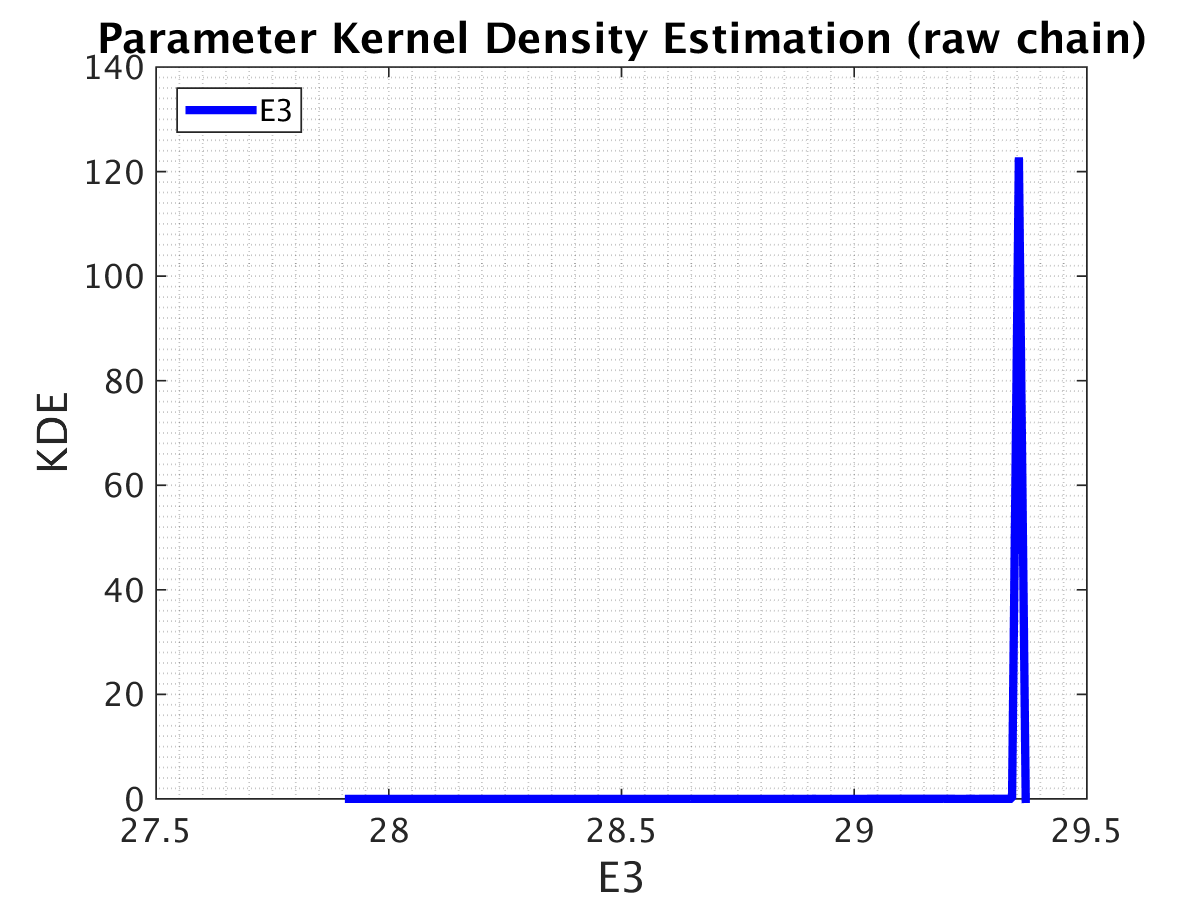
\includegraphics[scale=0.7]{one_parameter/1000_kde/outputData_1e6/simple_ip_kde_raw} 
            }  
\end{figure}
\begin{figure}[H]
 \ContinuedFloat
\centering
\subfloat[ LogLikelihood \label{subfig-1:dummy}]{
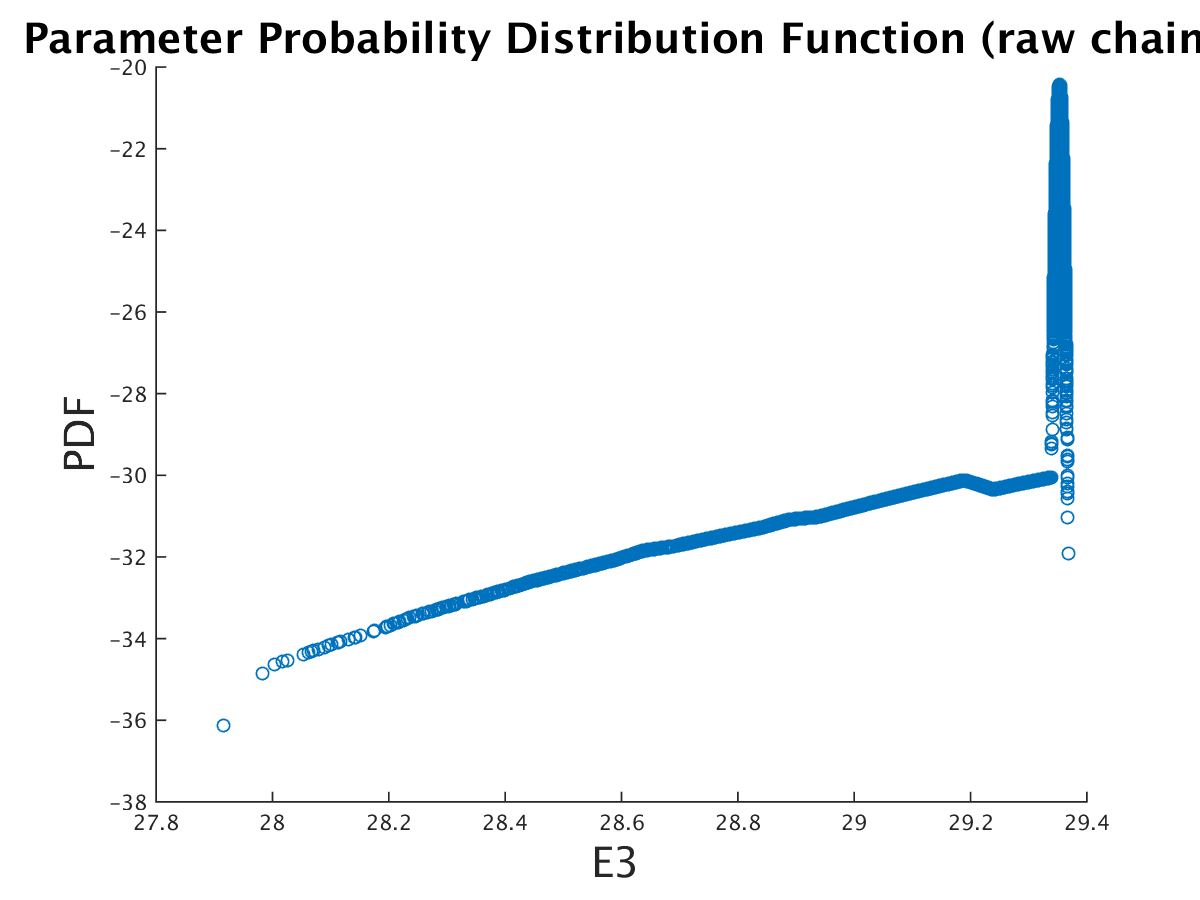
\includegraphics[scale=0.7]{one_parameter/1000_kde/outputData_1e6/ip_logLike_unified} 
  }
    \caption{Results for sample size 1e6}
\end{figure}


\begin{figure}[H]
\centering
\subfloat[MCMC raw chain of samples\label{subfig-1:dummy}]{%
     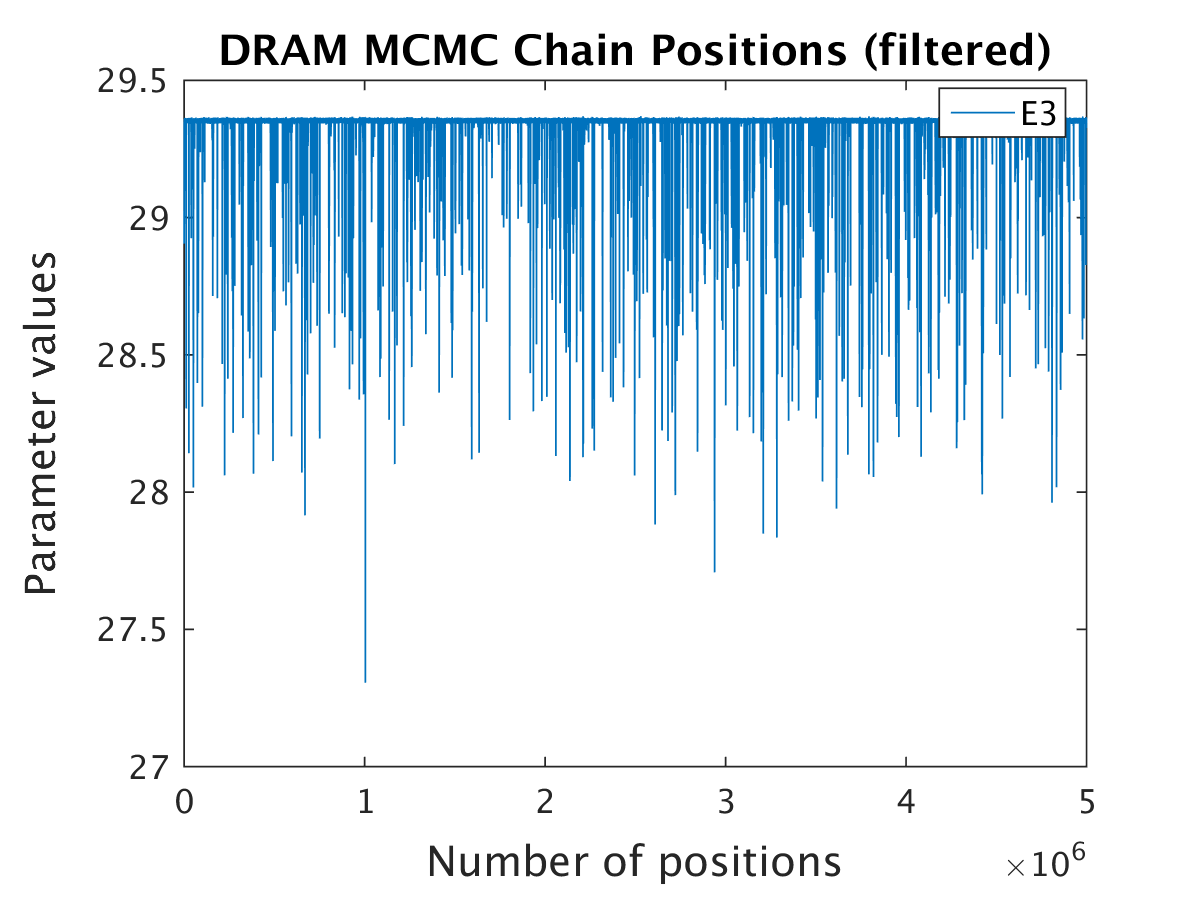
\includegraphics[scale=0.7]{one_parameter/1000_kde/outputData_5e6/simple_ip_chain_pos_filt} 
    }
    \quad
\subfloat[Histogram\label{subfig-1:dummy}]{%
     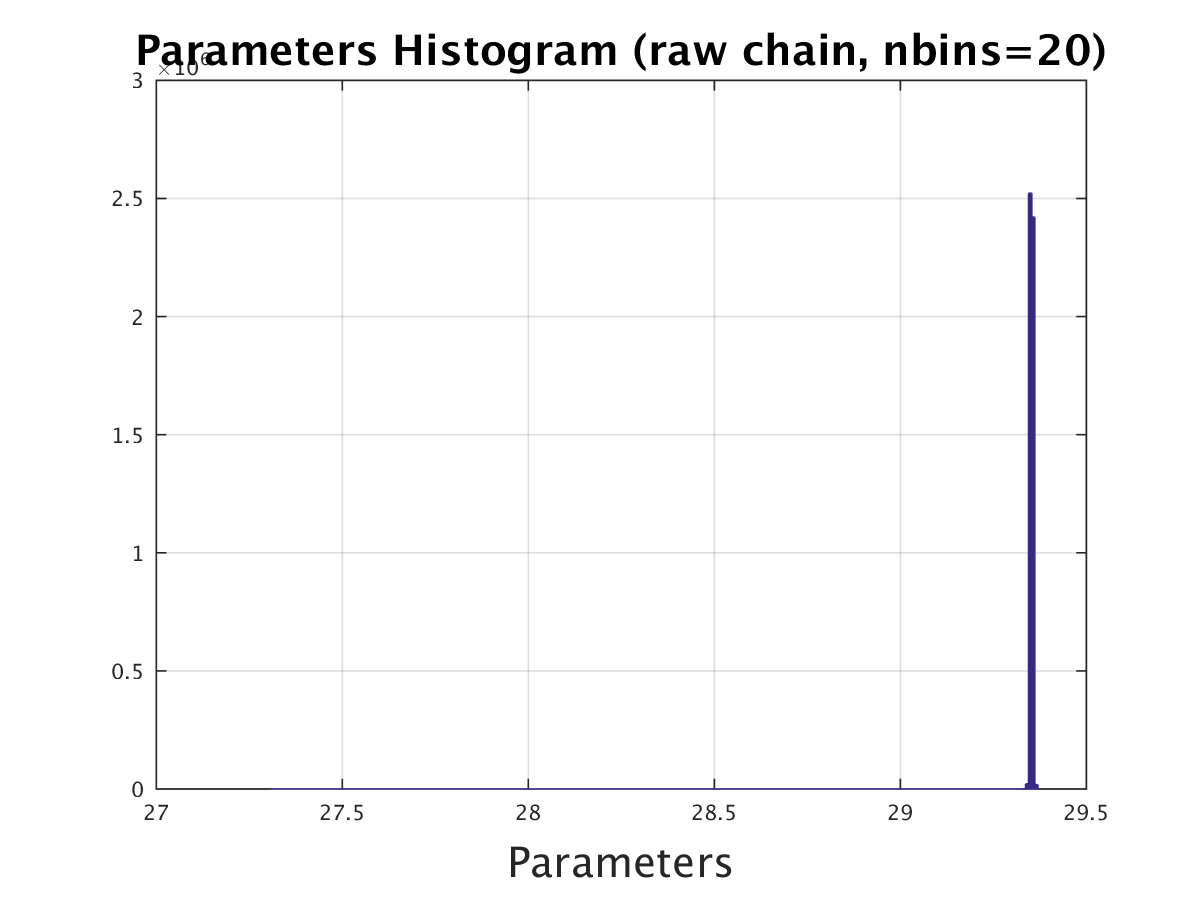
\includegraphics[scale=0.7]{one_parameter/1000_kde/outputData_5e6/simple_ip_hist_raw} 
    }
    \end{figure}
  \begin{figure}[H]
  \ContinuedFloat
  \centering
   \subfloat[Cummulative Density Funtion \label{subfig-1:dummy}]{
        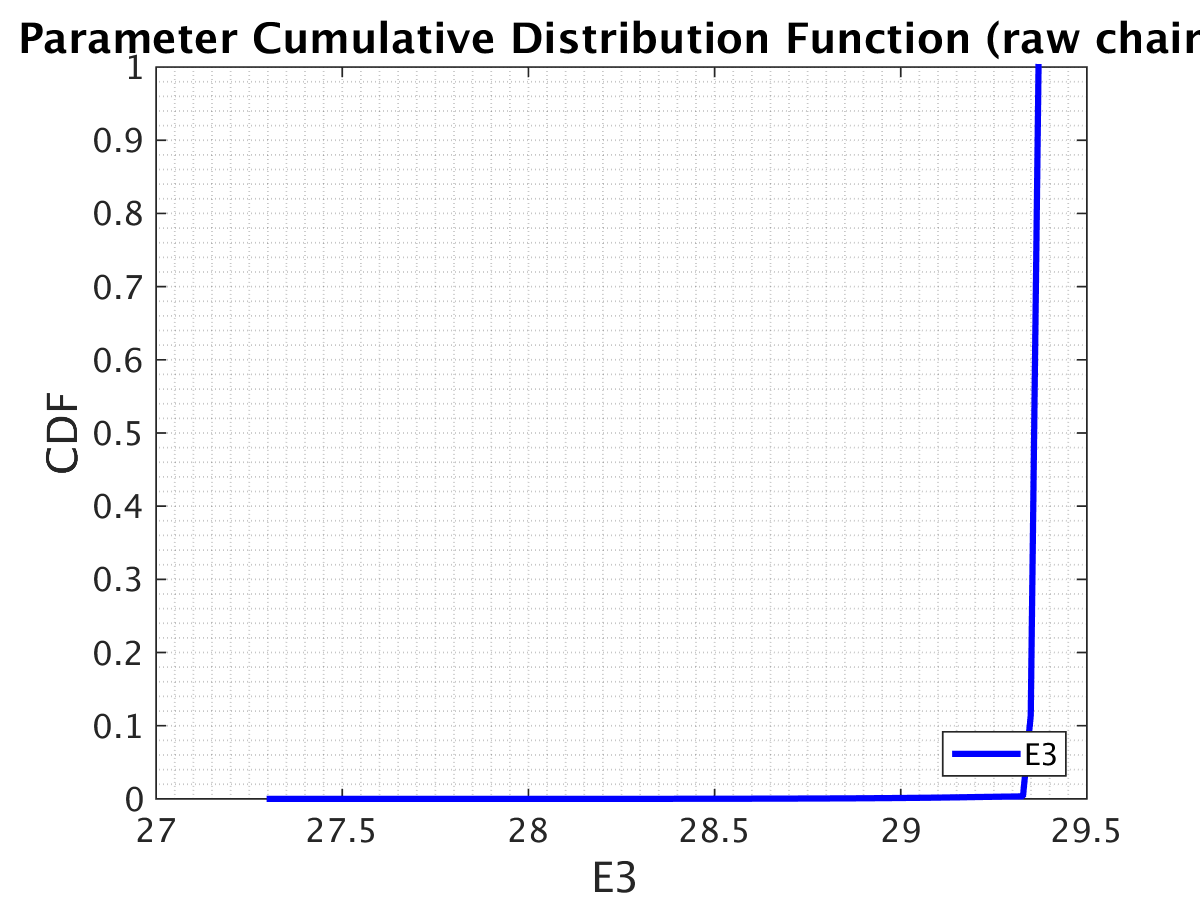
\includegraphics[scale=0.7]{one_parameter/1000_kde/outputData_5e6/simple_ip_cdf_raw} 
       }
     \quad
\subfloat[KDE \label{subfig-1:dummy}]{
        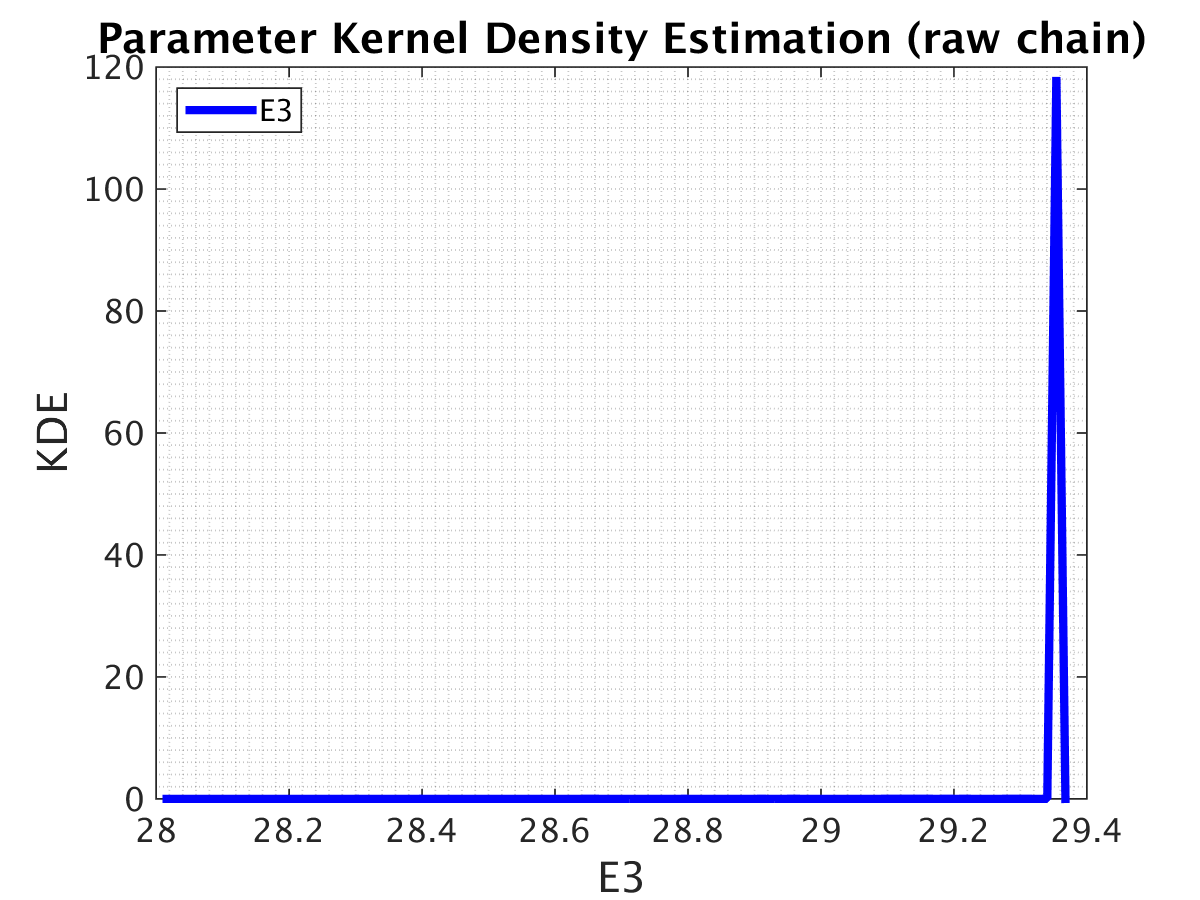
\includegraphics[scale=0.7]{one_parameter/1000_kde/outputData_5e5/simple_ip_kde_raw} 
            }  
\end{figure}
\begin{figure}[H]
 \ContinuedFloat
\centering
\subfloat[ LogLikelihood \label{subfig-1:dummy}]{
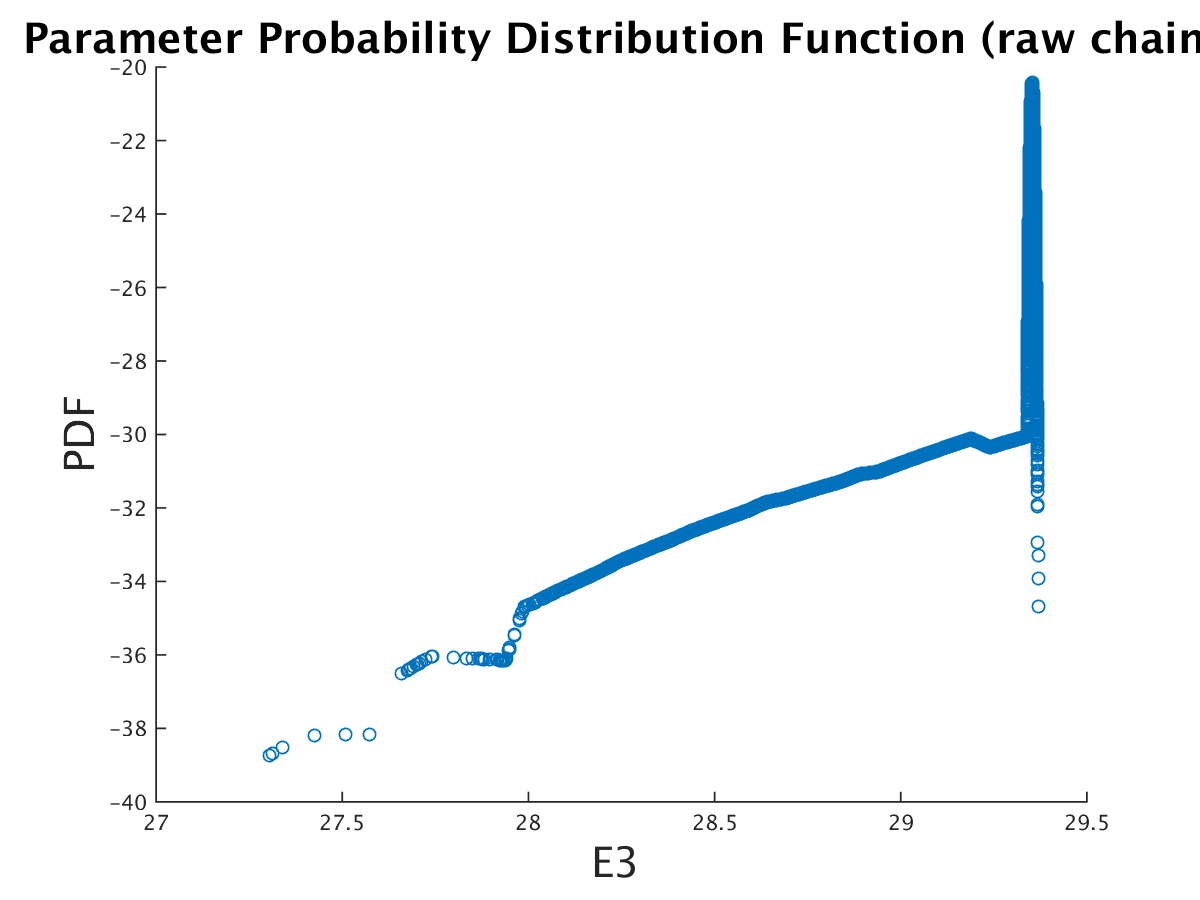
\includegraphics[scale=0.7]{one_parameter/1000_kde/outputData_5e6/ip_logLike_unified} 
  }
    \caption{Results for sample size 5e6}
\end{figure}



\begin{figure}[H]
\centering
\subfloat[MCMC raw chain of samples\label{subfig-1:dummy}]{%
     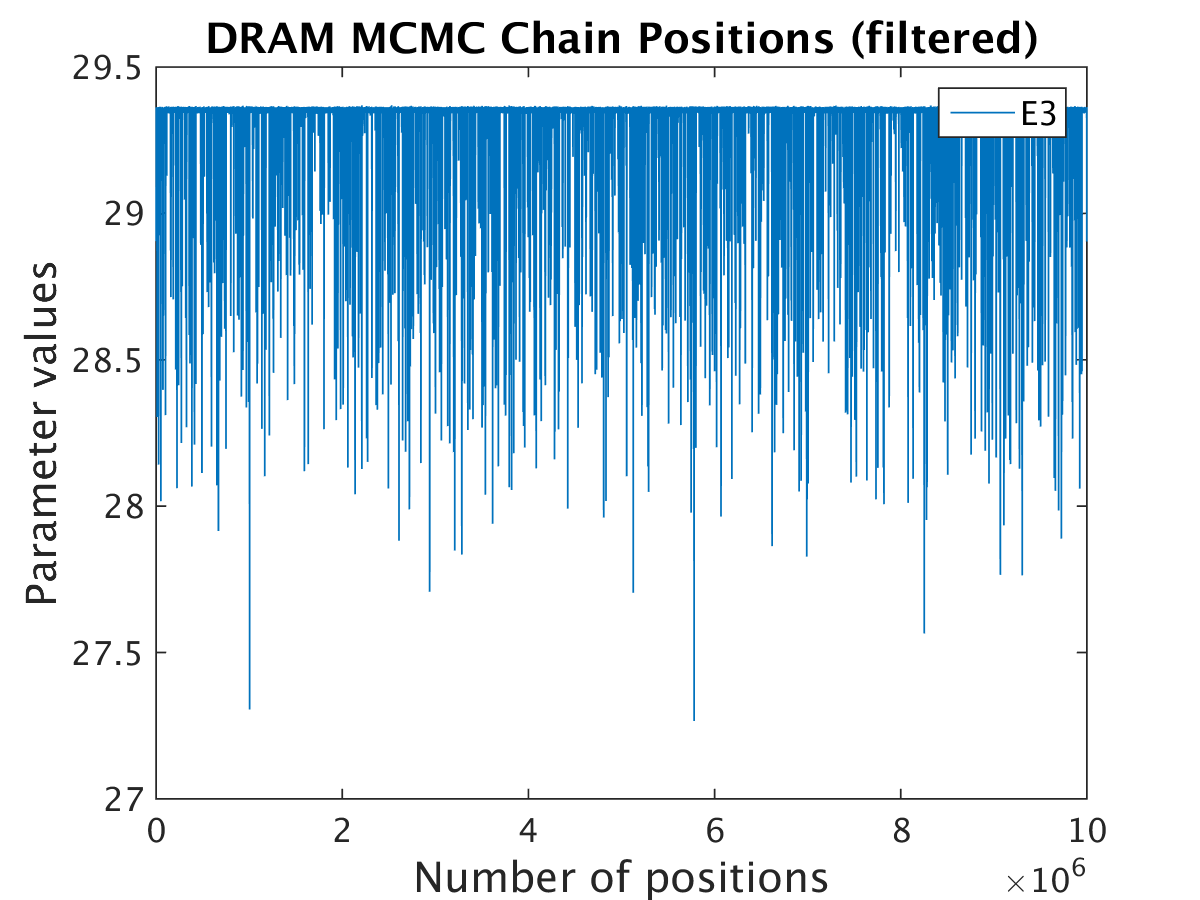
\includegraphics[scale=0.7]{one_parameter/1000_kde/outputData_1e7/simple_ip_chain_pos_filt} 
    }
    \quad
\subfloat[Histogram\label{subfig-1:dummy}]{%
     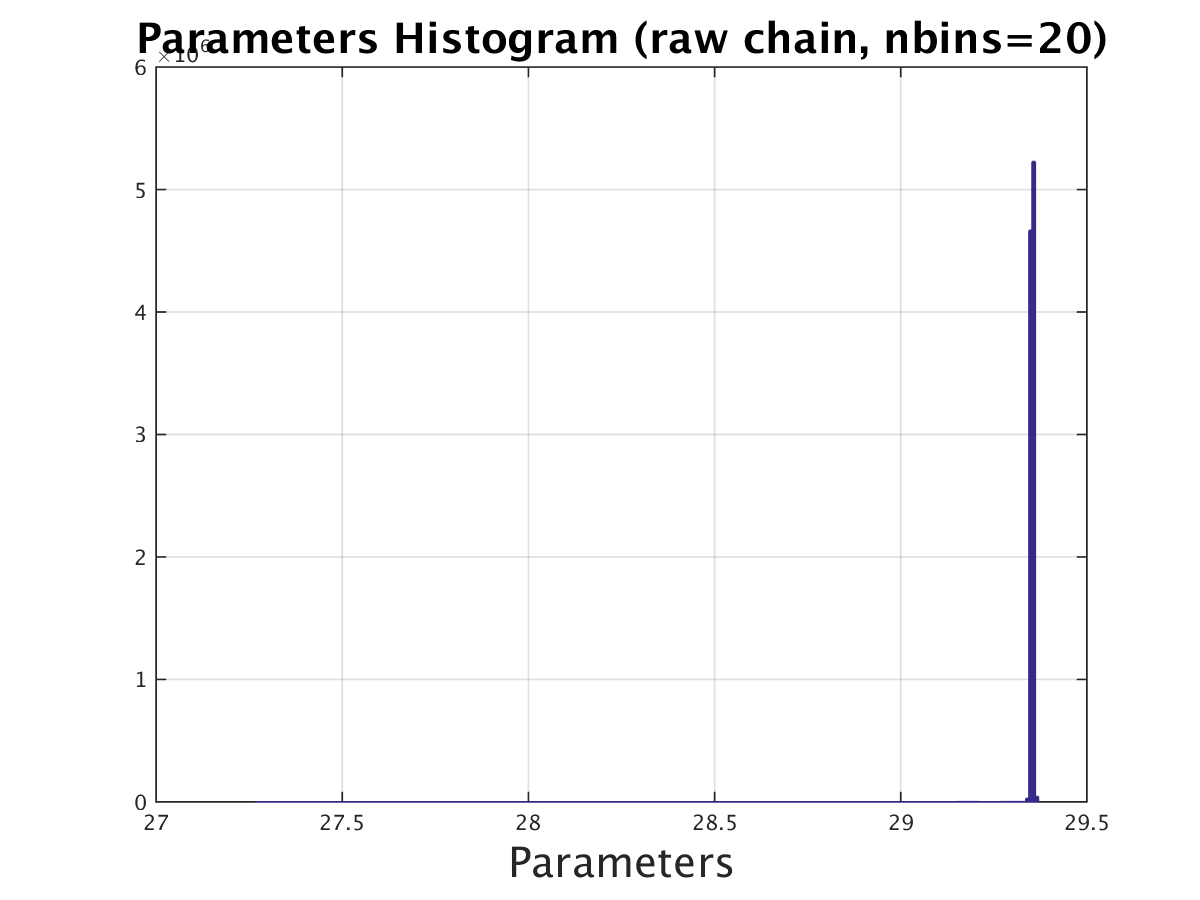
\includegraphics[scale=0.7]{one_parameter/1000_kde/outputData_1e7/simple_ip_hist_raw} 
    }
    \end{figure}
  \begin{figure}[H]
  \ContinuedFloat
  \centering
   \subfloat[Cummulative Density Funtion \label{subfig-1:dummy}]{
        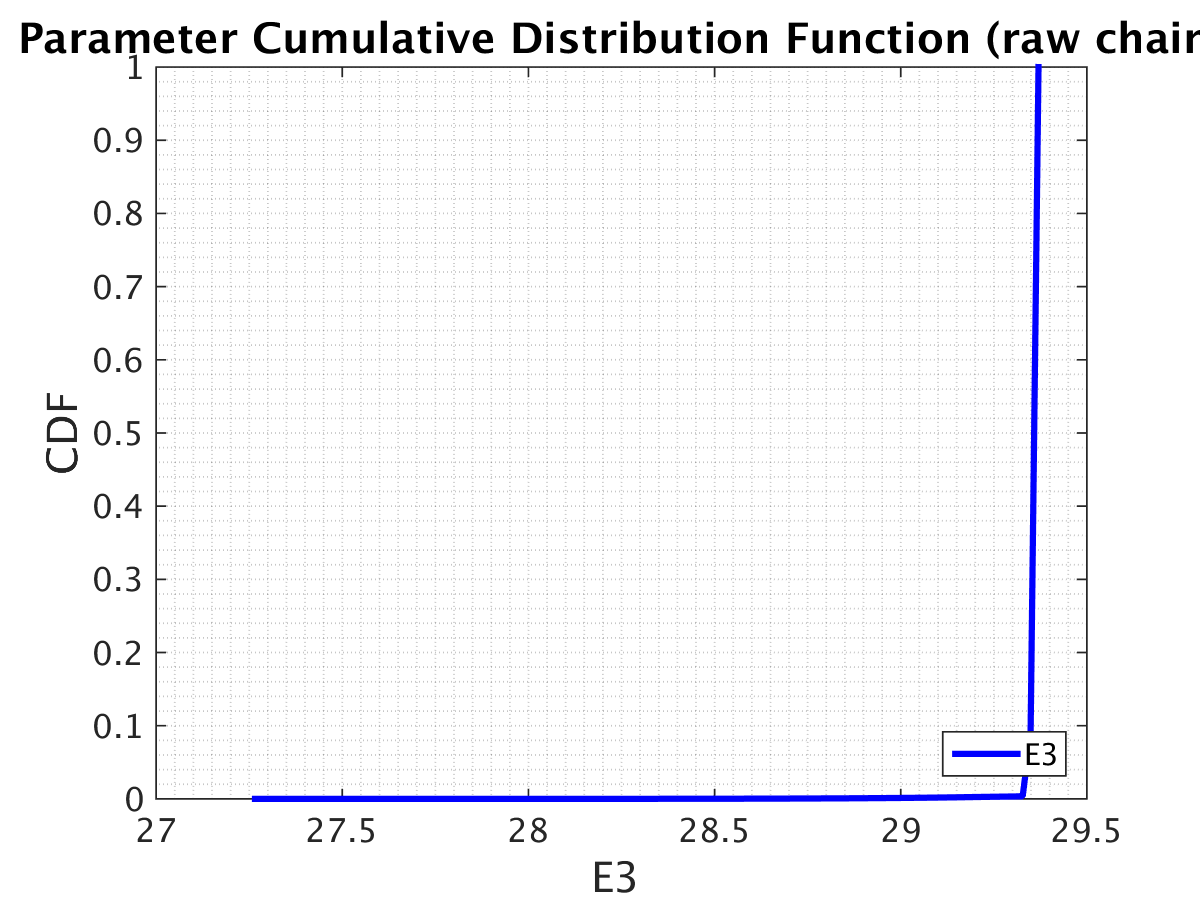
\includegraphics[scale=0.7]{one_parameter/1000_kde/outputData_1e7/simple_ip_cdf_raw} 
       }
     \quad
\subfloat[KDE \label{subfig-1:dummy}]{
        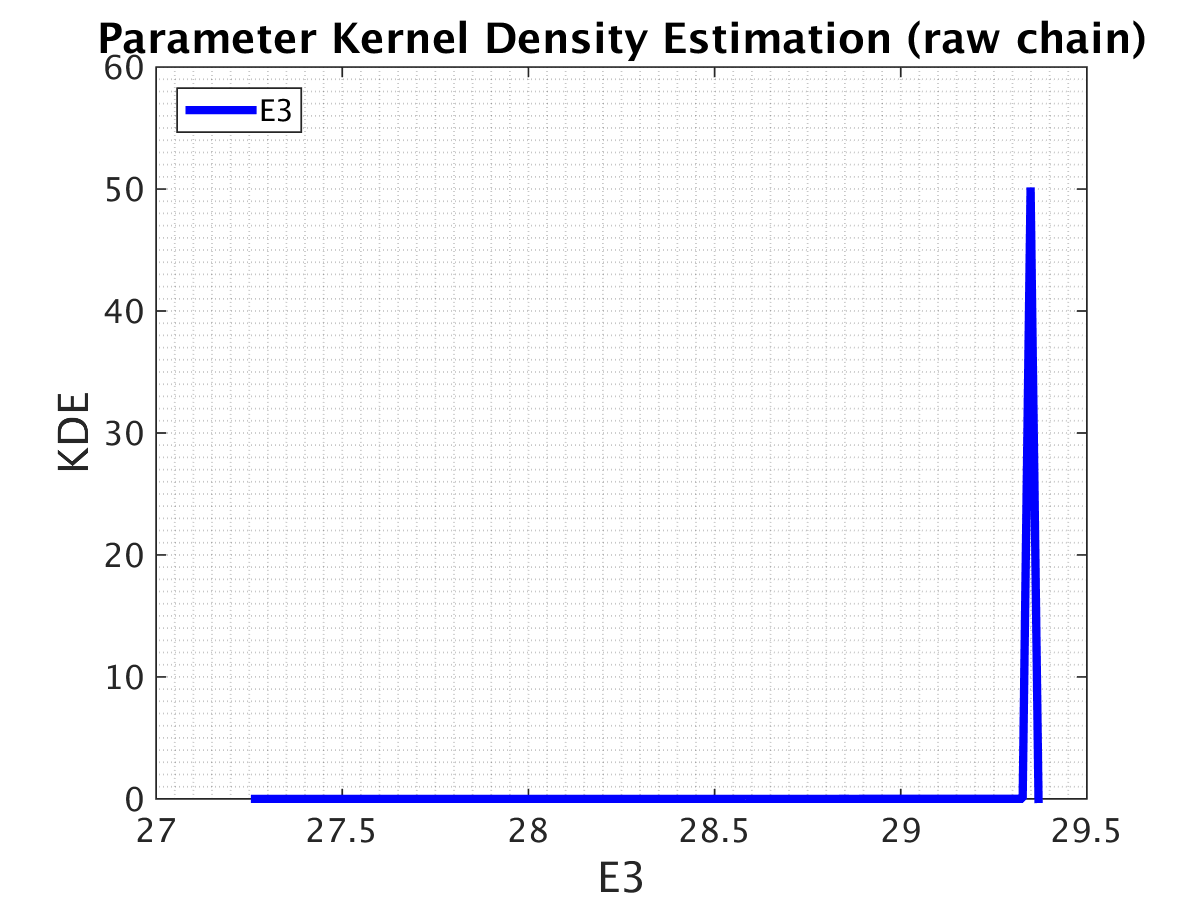
\includegraphics[scale=0.7]{one_parameter/1000_kde/outputData_1e7/simple_ip_kde_raw} 
            }  
\end{figure}
\begin{figure}[H]
 \ContinuedFloat
\centering
\subfloat[ LogLikelihood \label{subfig-1:dummy}]{
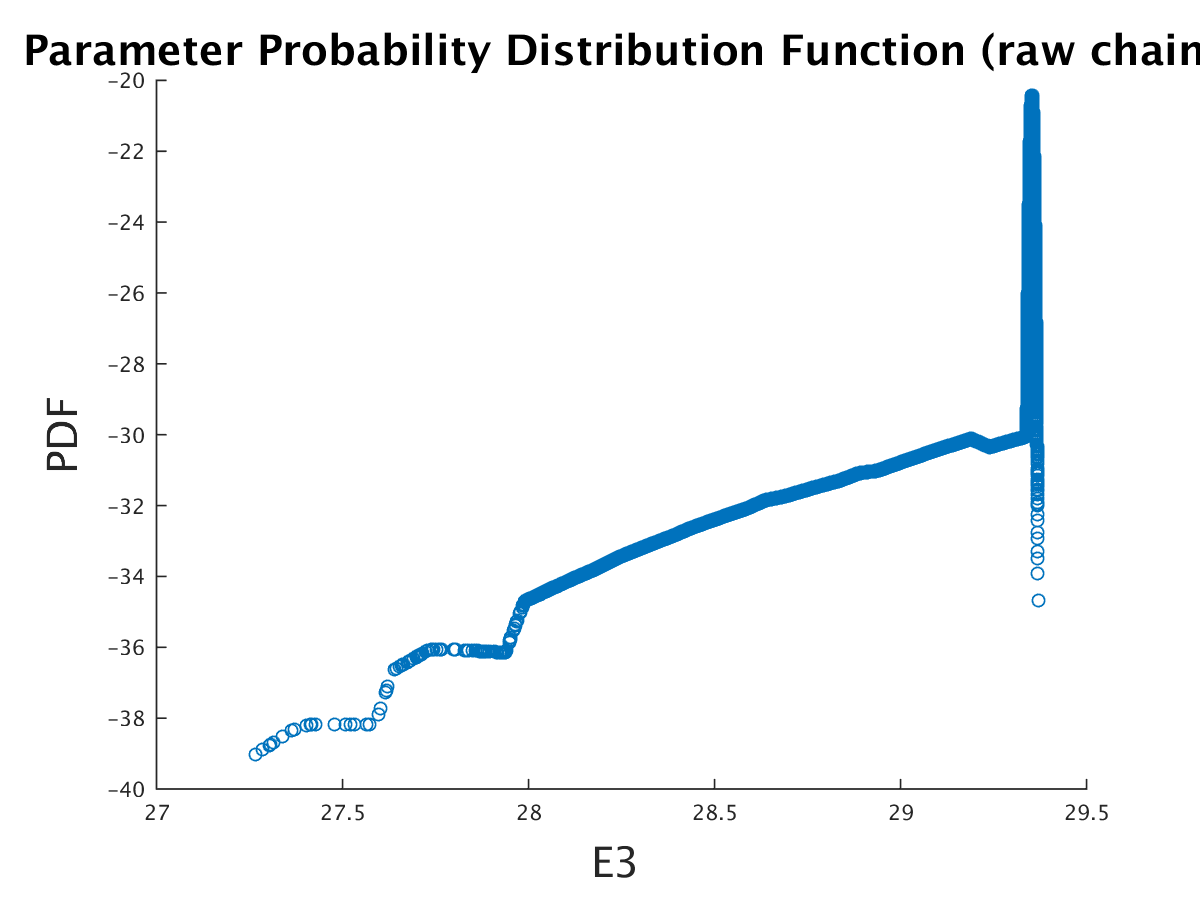
\includegraphics[scale=0.7]{one_parameter/1000_kde/outputData_1e7/ip_logLike_unified} 
  }
    \caption{Results for sample size 1e7}
\end{figure}